\chapter{Overall System Design}

\section{Media Consumption Control System} %name our system
The Media Consumption Control System (MCCS) is the system that are our solution on the problem statement. To give an overview of the complete system a rich picture have been made, see the figure \ref{fig:systemoverview}. The figure show a home environment with a TV (media), computer and a internet connection, and it show a server. 

There are two main use pattern. The first is a parent who manage the their MCCS and uses the website from the PC to add, change or delete settings. This is pictured in the bottom left-side corner in figure \ref{fig:systemoverview}. 

The second use pattern is pictured in the upper left corner of the figure. It is a child user who want to use a media and in this case watch television, but to see television power is needed and its power source is blocked by the controller. So the child need to scan his tag and then the controller sends a message to the server which then reply whether the television can be turned on. When the child is done he must scan again such that points can be withdraw from his user profile. When the child does not have any point he cannot turn on the television nor can he if a rule or permission do not allow it. If a parent wants to watch television without being restricted in any way he can make a rule that gives him unlimited access, but he would still need to scan his tag before and after using the television.

\begin{figure}
	\centering
		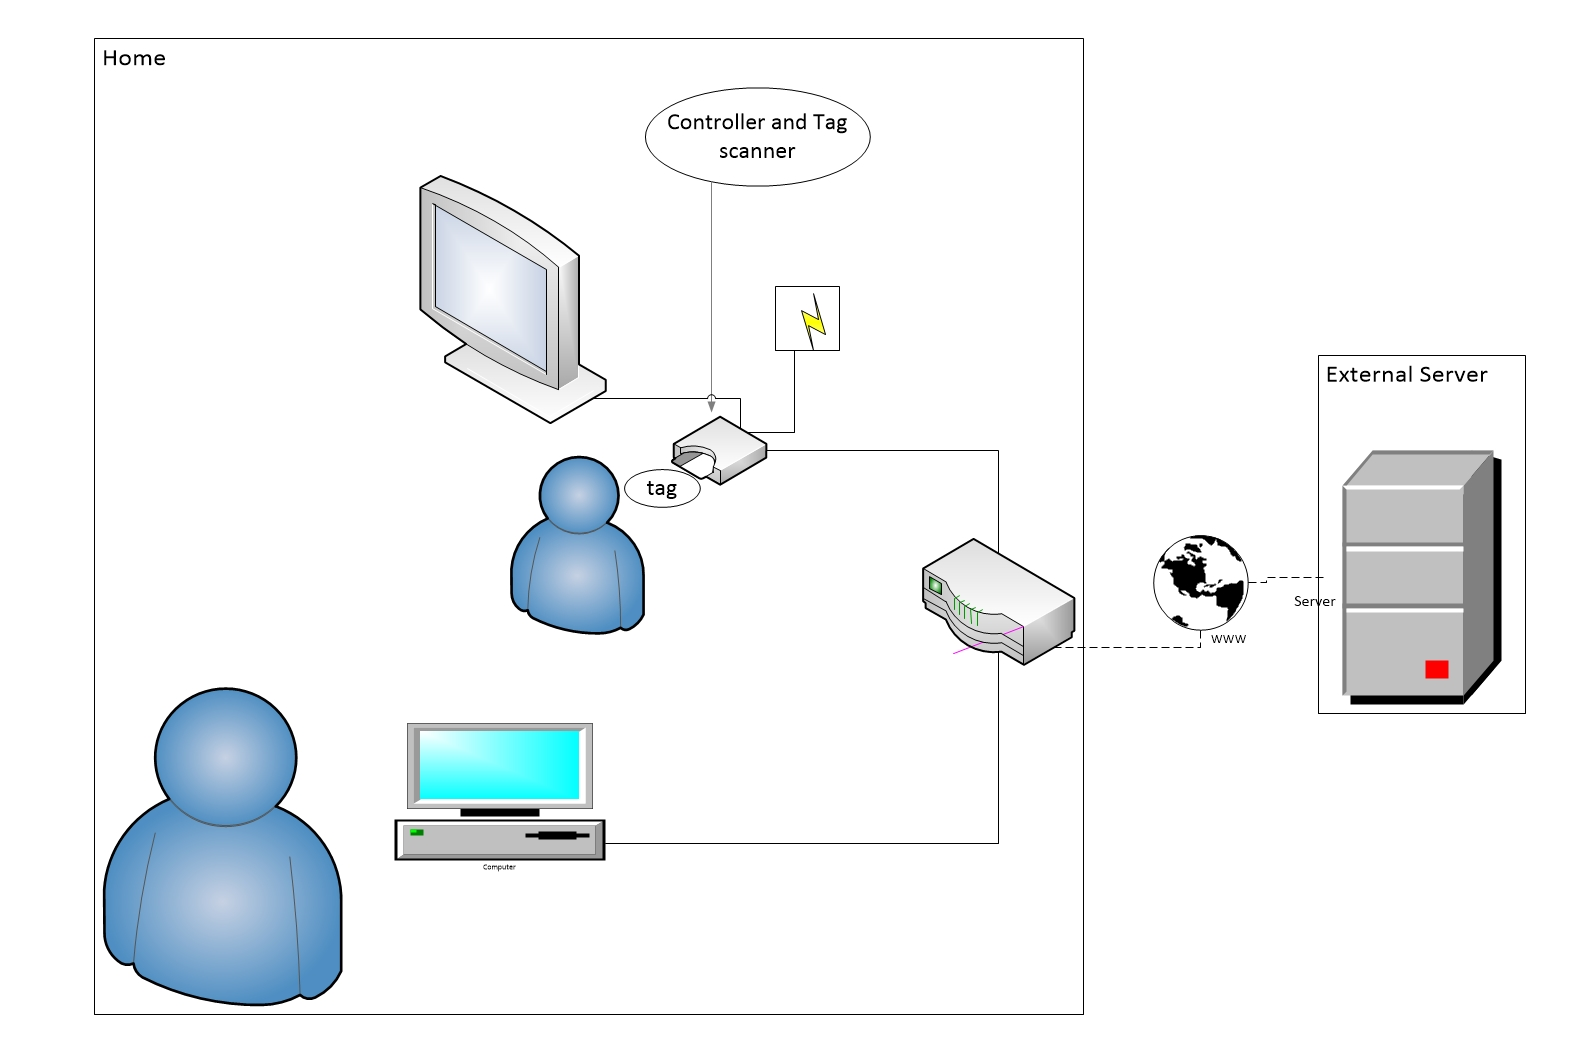
\includegraphics[width=1.00\textwidth]{images/systemoverview.jpg}
	\caption{system overview}
	\label{fig:systemoverview}
\end{figure}

This is how the MCCS is supposed to work but some hardware and requirements to the system is needed. Previously we came to the conclusion that the following is needed.
\begin{itemize}
	\item A device to toggle the power of an electronic media
	\item An individual key for each child that can be read by the device
	\item A web-interface to set up rules, permissions and view/modify allowed usage of electronic media
\end{itemize} 

The first item is in the figure called a controller, the second is called a tag and the last is the website on the computer. In the following sections their specification will be explained further together with the decision of which hardware that are to be used. 
\subsection{Tag and Controller}
The tag used in this system is using Radio-frequency Identification (RFID). The tag need to be uniquely identified in the MCCS and it must uniquely identify its user. The tag is used in combination with the controller.

The controller is a reader and an Arduino in this system and like the tag it need to be uniquely identified in the MCCS. The controller must be able to:

\begin{itemize}
	\item read the data from the tag
	\item send messages to the servers API
	\item temporary store the user that uses this controller
	\item keep track of the time spent between the media usage began to it end
\end{itemize}
 

\subsection{MCCS's Website}




%Symbolise use: TV, Controller, Reader, Tag, Child, Network Con, Laptop, Parent, Server
%
%Pull the list from the analysis and explain what we need to implement these features.
%\begin{enumerate}
	%\item A way to set up permissions for which media and when they can be accessed
	%\item A way to set up rules to make exceptions to these permissions
	%\item A way to monitor/limit the usage of media used by a child
	%\item A way to uniquely identify the child in the physical world
	%\item A way to inspire children to physical activity
%\end{enumerate}
%

%This idea then boils down to these 3 key aspects:
%
%\begin{itemize}
	%\item A device to toggle the power of an electronic media
	%\item An individual key for each child that can be read by the device
	%\item A web-interface to set up rules, permissions and view/modify allowed usage of electronic media
%\end{itemize} 


\section{general concepts}
%Go into detail about rules, permission, chores
\subsection{Rule}
\subsection{Permission}
\subsection{Chores}


\section{System architecture}
%Symbolise server: API, Website, Daemon, Server, connection to controller, connection to laptop




